\documentclass[sigconf,anonymous=true]{acmart}

\usepackage{booktabs} % For formal tables

% Copyright
\setcopyright{none}
%\setcopyright{acmcopyright}
%\setcopyright{acmlicensed}

%\setcopyright{rightsretained}

%\setcopyright{usgov}
%\setcopyright{usgovmixed}
%\setcopyright{cagov}
%\setcopyright{cagovmixed}

\settopmatter{printacmref=false}


% DOI
\acmDOI{}

% ISBN
\acmISBN{}

%Conference
\acmConference[ACSAC'18]{Annual Computer Security Applications Conference}{December 2018}{San Juan, Puerto Rico}
\acmYear{2018}
\copyrightyear{2018}

\acmArticle{}
\acmPrice{15.00}

% These commands are optional
%\acmBooktitle{Transactions of the ACM Woodstock conference}
\editor{}
\editor{}
\editor{}


\begin{document}
\title{Detection Methods for Distributed Web-Crawlers: Long-tail Threshold Model}
%\titlenote{Produces the permission block, and copyright information}

\author{Inwoo Ro}
\orcid{1234-5678-9012}
\affiliation{%
  \institution{Hanyang University}
  \streetaddress{P.O. Box 1212}
  \city{Seoul}
  \country{Korea}
  \postcode{43017-6221}
}
\affiliation{%
  \institution{NAVER WEBTOON Corp.}
  \streetaddress{P.O. Box 1212}
  \city{Bundang}
  \country{Gyeoungi-do}
  \postcode{43017-6221}
}
\email{inwoo13@hanyang.ac.kr}

\author{Joong Soo Han}
\affiliation{%
  \institution{Hanyang University}
  \city{Seoul}
  \country{Korea}
  \postcode{43017-6221}
}
\email{soohan@hanyang.ac.kr}

\author{Eul Gyu Im}
\orcid{0000-0002-4130-513X}
\affiliation{%
  \institution{Hanyang University}
  \city{Seoul}
  \country{Korea}
  \postcode{43017-6221}
  }
\email{imeg@hanyang.ac.kr}

% The default list of authors is too long for headers.
%\renewcommand{\shortauthors}{B. Trovato et al.}


\begin{abstract}
In this paper, we propose an advanced countermeasure against distributed web-crawlers. We investigate the state of the art methods for crawler detection and analyze how distributed crawlers can bypass these methods.  Our method can detect distributed crawlers by focusing on the property that web traffics follow the power distribution. When we sort the items by the number of requests, most of the requests are concentrated on the most frequently requested items. In addition there will be an area that normal users are not generally request. But crawlers will request for it because of their algorithms are intend to request iteratively by parsing web-pages to collect every items they aimed for. By following these two properties, we can assume that if some IPs are frequently requesting the items that are located in longtail area, those IPs can be classified as crawler node. The experimental results with NASA web-traffic data showed our method was effective for identifying distributed crawlers with low false positives.
\end{abstract}


\keywords{Web Crawler, Traffic Analysis, Power Law, Information Theory}

\maketitle


%
% Introduction
%
\section{Introduction}
Web-crawling is used in various fields for collecting data[1]. Some web-crawlers collect data even though the target site is prohibiting crawlers by robot.txt. Some web services try to detect and prevent crawlers by anti-crawler methods but these malicious web-crawlers bypass detection by modifying their header values or distributing IPs to masquerade as if they are normal users.
It is a matter of availability and data property issue because even though any service allows users to access each data, it is prohibited to duplicate the entire dataset. And malicious web-crawlers can cause significant traffic and intellectual property infringement by collecting the entire data from web services. This can cause a serious impact on the availability of the target service.
In this paper, we investigate the conventional anti-crawling methods and its countermeasures, and show that the conventional anti-crawling methods cannot stop distributed crawlers. Then we propose the new anti-crawling technique that we call LTM(Long-tail Threshold Model) which gradually adds the distributed crawler node IPs to the block-list.

%
% Back Ground
% with 2 subsections
%
\section{Related Works}
In this section, we will summarize conventional anti-crawling methods and their counter crawling measures.

\begin{itemize}
\item HTTP Header Check\newline
A basic crawler will send requests without modification on its header information. Web servers can distinguishes a legitimate user from a crawler by checking the request header, especially if the User-Agent value has been set properly. This header checking method is a basic anti-crawling method[10].
However if a crawler attempts to masquerade itself as a legitimate user, it will replay the header information from the web browser or form the http header information similar to a browser. This makes it difficult for a web server to determine whether a client is a crawler or a legitimate user by simply checking the request header.

\item Access Pattern based Anti-Crawling\newline
Access pattern based anti-crawling is a method of classifying legitimate users and crawlers based on the pattern requested by the client. If a client requests only a specific resource continuously without a call to a resource that should normally be requested, the client will be regarded as a crawler. 
A crawler performing an aggressive crawling predefines the core data that the crawler wants to collect, and requests specific data without requesting unnecessary resources. In this case, the web server can recognize that the client is not a legitimate user.
In the case of a web service using access pattern recognition, the service analyzes the pattern when a normal user accesses through the UI. If some requests have a significant difference from this pattern, the service classifies it as a crawler[10].
Although this approach can recognize a crawler based on access pattern, some crawlers even masquerade their access pattern by analyzing network logs[4].

\item Access Frequency based Anti-Crawling\newline
Access frequency based anti-crawling is a method that determines a client is whether a crawler or a legitimate user by access frequency rate. A web server can set a threshold, the maximum number of access in a specific time window. If a client issues requests more than this threshold within the pre-defined time, the web server determines that the client as a crowler[4].

This method has two well-known problems. 
First, it has a vulnerability against distributed crawlers. If an attackers use distributed crawlers such as Crawlera, the access rate of each crawler node can be managed enough to stay lower than the threshold.
Second, there is a chance to detect normal users sharing a public IP as crawlers.
\end{itemize}


%
% BLOCKING DISTRIBUTED CRAWLER
% with 2 subsections
%
\section{BLOCKING DISTRIBUTED CRAWLER}
As described in previous section, distributed crawler can bypass every conventional anti-crawling methods. In this section, we propose a new technique to detect and block distributed crawlers that could not be defended by conventional anti-crawling techniques.

\subsection{Required Number of Crawler Nodes}
In order for the Distributed crawler to collect the entire data of a website, the following conditions must be met.

\begin{displaymath}
Cn \geq Um / (Td * 30) 
\end{displaymath}

The above formula can be described as follows.

\begin{itemize}
\item Um: Number of items updated in month
\item Td: Maximum number of request per IP
\item Cn: Number of crawler node(IP)
\end{itemize}

For an example, if there is a web service updates Um(30,000) items in a month and the service has a restriction rule that if an IP requests more then Td(100) times will be blocked and an attacker who tries to collect every items from the service will need Cn(10) crawler nodes to avoid restriction.
Therefore, as Um increases or Td decreases, Cn increases. And Cn numerically indicates the level at which the website is difficult to crawl.

\subsection{Generating Long-tail Td zone}
The number of items that are updated in a month can not be arbitrarily increased. Therefore, simple way to prevent distributed crawler is to decrease Td. But this will also increase false positive significantly. In this paper, we solve this problem by reversing the general characteristics of web traffic and the fact that the crawler tries to replicate the entire data.
If you sort the items by access rate, you can see the exponentially decreasing form as shown in the following figure. This means most of the web traffic is concentrated on most frequently requested items. And there is a long-tail region that has low access rate. We calculated max request count of this longtail region and set this value as Td3.

\begin{figure}[H]
    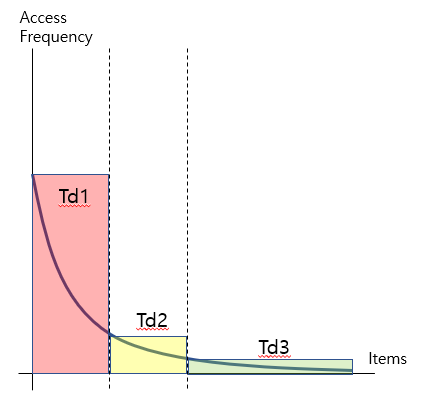
\includegraphics[width=0.7\columnwidth]{figs/figure_01.png}
    \caption{Access Frequency per number of connections}
    \label{fig:fig1}
\end{figure}

In information theory, unlikely event is more informative then likely event. And the event that a request to an item in long-tail region is much unlikely then the upper items. This means the web service can find more information from a request to the long-tail region.
Hence, when a client keep request the items in long-tail region, the web service increase the count until it reaches Td3, instead of reaching Td mean. This means a web service can set much more sensitive threshold without increasing false positive error rate.


\subsection{Node Reducing with Long-tail Region}
In order for an attacker to collect the entire data from the service, he or she must also access the items in the long-tail (Td3) interval. However, the attacker does not know exactly which item the item he is accessing belongs to. Using this information asymmetry, service providers can easily identify IPs that are accessed more frequently than long-tailed segments. These identified crawler IPs will included in block-list and the number of IPs in blcok-list will be called Cm. If we start to increase the Cm value through the long-tail interval, the attacker will crawl with a smaller number of IPs, and Cm will increase in the Td3 interval.

\begin{itemize}
\item Cm: Number of crawler node(IP) blocked by service
\item long\_t: Ratio of items included in long-tail region
\end{itemize}

So attackers must satisfy the following inequality. Cn - Cm is the number of non-blocked crawler nodes and this should be greater then the right term.

  \begin{displaymath}
Cn - Cm \geq (Um * long\_t) / (Td3 * 30)
  \end{displaymath}

On the service provider side, Cm should be greater then right term to block distributed crawlers.

  \begin{displaymath}
Cm > Cn - (Um * long\_t) / (Td3 * 30)
  \end{displaymath}

If a particular IP accesses an item in the long-tail region with more than the Td3 value determined by the above formula, it can be included in the block-list.


\subsection{Dummy Items}
The service provider may include a dummy item to detect the crawler in addition to the actual service target item. Dummy items are inaccessible for the legitmiate user because there are no user interfaces for dummy items or hidden. There are few ways to generate dummy items, it may exists as an HTML tag but it is not displayed on the screen by the attribute setting or it may contains a garbage information that normal users shell not be interested. But a crawler that performs sequential access to the service will may access the dummy items. By this characteristic, dummy items can work as extension of the long-tail region.

In this paper, we will not include dummy items in experiments due to fair comparsion with real traffic logs which will not access dummy items.



%
% EXPERIMENT
% 1. Web Traffic Data
% 2. Simulation
% 3. Node Reducing Result
%
\section{EXPERIMENT}
Our experiment was designed to verify the classification performance of crawler detection module between crawlers and legitimate  web traffics. We compared LTM(Long-tail Threshold Model) with normal access frequency based anti-crawling on maximum number of crawler nodes and false positive.
We used the real web traffic log that NASA released in 1995. And then we performed pre-processing, modeling and simulation.

\begin{figure}[H]
    \centering
    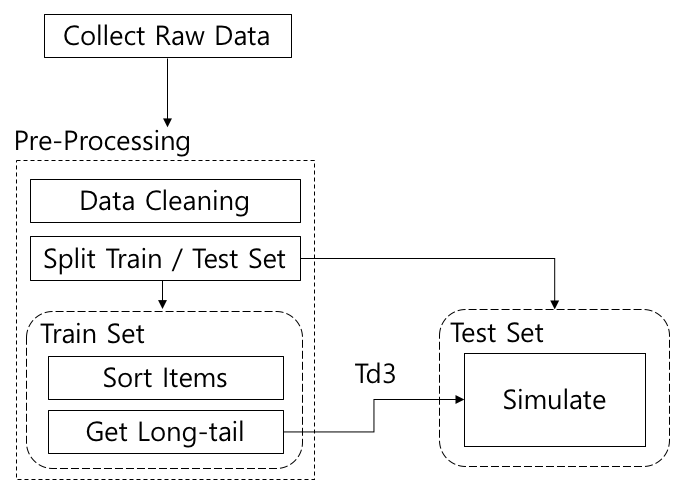
\includegraphics[width=0.85\columnwidth]{figs/figure_design.png}
    \caption{Experiment Design}
    \label{fig:fig2}
\end{figure}


\subsection{Web Traffic Data}
\begin{itemize}
\item Source\newline NASA released a total of 1,891,715 access logs for the month of July 1995. We parsed this log into csv format and composed of 4 columns including IP, date, access target and access result.
The total number of connected IPs are 81,978 and the number of items are 21,649.\newline

\item Data Pre-Processing and Traffic Distribution\newline In order to prevent duplication of data used for in modeling and experimental data in the time series data, we split the log by time. July 1 to 24 was used for LTM modeling and 25 to 30 was used for testing.
When a user accesses a html file, they also get accesses to gif files that are linked. This can force a multi increase of access count. Hence we removed some gif files from the long-tail. In addition, we excluded the request logs that the access results are not success from the experiment. After doing the pre-processing we have got the test set as below table.

\begin{table}[H]
  \caption{Pre-Processed Web Traffic Data}
  \label{tab:freq}
    \begin{tabular}{| p{3.1cm} | p{2cm} |}
    \hline
    Number of Total Items & 7,649 \\ \hline
    Number of Long-tail & 5,355 \\ \hline
    Mean of Total Items & 184.76 \\ \hline
    Mean of Long-tail & 1.88 \\ \hline
    \end{tabular}
\end{table}

As a result, we made a pre-processed traffic data set consists of 7,649 items from 21,649 raw data. Which has 5,355 items as a long-tail region. The mean of the total request count was 184.76, and the mean of long-tail region was 1.88. It means simply we can set about 6880\% more sensitive threshold to the crawler detection algorithm.

\begin{table}[H]
  \caption{Experiment Data}
    \begin{tabular}{| l | l | l | l | l | }
    \hline
    & Ratio & mean & max & count \\ \hline
    Td1 &  > 0.5\% & 21,250 & 76,040 & 38 \\ 
    Td2 & 0.5\% - 30\% & 264 & 7,043 & 2,256 \\
    Td3 & 30\% > & 1.88 & 9 & 5,355 \\ \hline
    \end{tabular}
\end{table}
The key part of the experiment was simulating with the real web traffic data. We checked whether the NASA data reperesent power distribution after sorting with access frequency or not. And we could verify the traffic also has power distribution as shown in Figures 2, 3 and 4.
\end{itemize}

\begin{figure}[H]
    \centering
    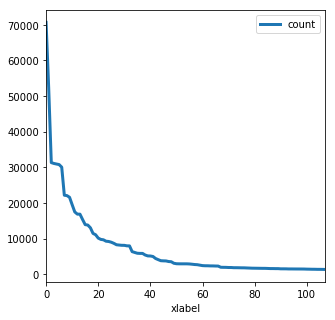
\includegraphics[width=0.85\columnwidth]{figs/figure_02_td1.png}
    \caption{Access Count in Td1}
    \label{fig:fig3}
\end{figure}
Figure 2 shows the group of the most frequently requtestd items. 

\begin{figure}[H]
    \centering
    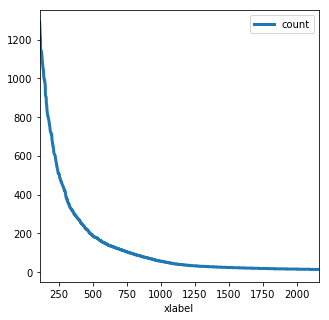
\includegraphics[width=0.85\columnwidth]{figs/figure_03_td2.png}
    \caption{Access Count in Td2}
    \label{fig:fig4}
\end{figure}

\begin{figure}[H]
    \centering
    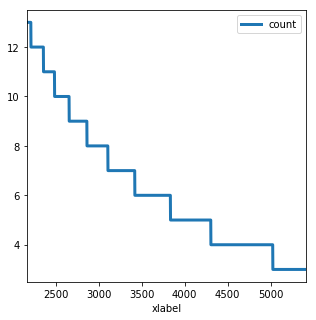
\includegraphics[width=0.85\columnwidth]{figs/figure_04_td3.png}
    \caption{Access Count in Long-tail}
    \label{fig:fig5}
\end{figure}

Figure 4 shows the long-tail region of sorted result. We set Td3 threshold value as 20 which is about 2 times larger than the maximum access rate of long-tail region. Setting a Td3 value in LTM has a heuristic part because web services has different purposes and circumstances.

\subsection{Simulation}
In this paper, we implemented simulation for two purpose. One is to check whether LTM would be able to detect and disable a distributed crawler IP group and the other one is to check false positive when input the actual web traffic to LTM.

\begin{figure} [H]
    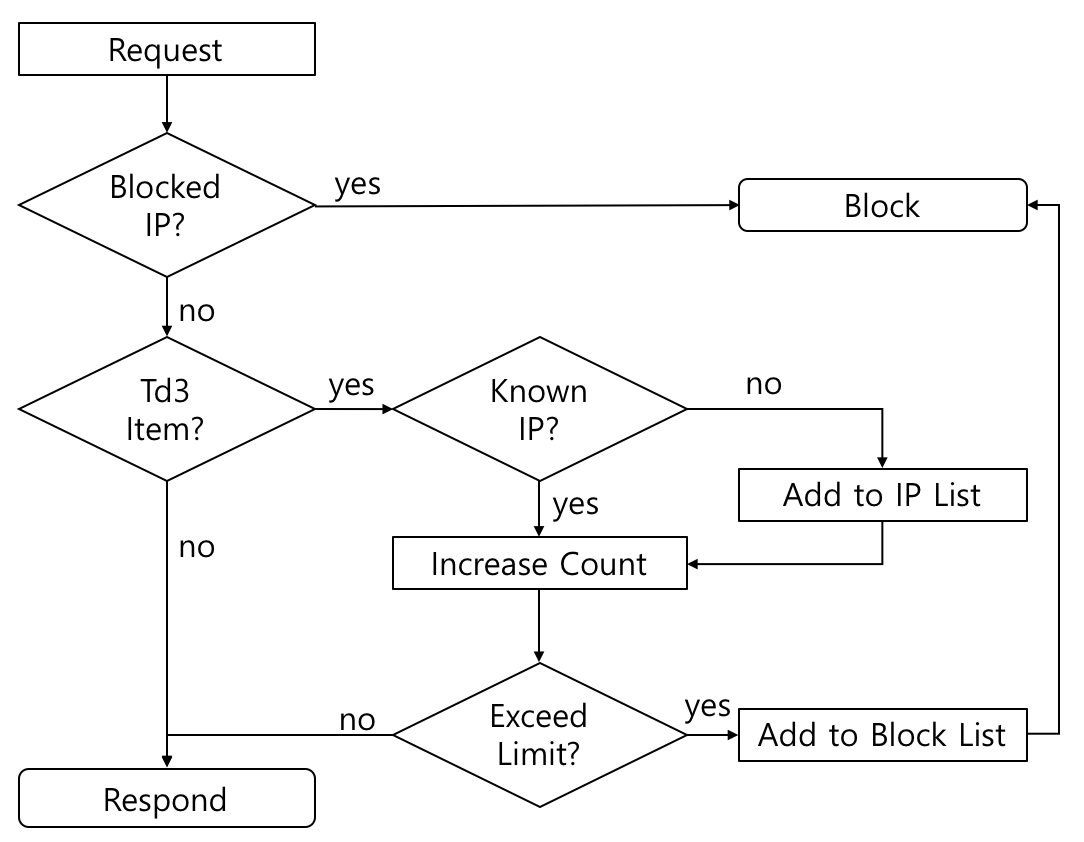
\includegraphics[width=0.88\columnwidth]{figs/flow_chart_01.png}
    \caption{Crawler Detection Flow}
    \label{fig:fig6}
\end{figure}


\begin{itemize}
\item Distributed Crawler Detecting Simulation\newline We used python for implementing the LTM simulator. The required parameters are 1) the size of the distributed IP set used by the crawler, 2) the long-tail list, 3) the entire item list, and 4) threshold values used for detection.
The LTM simulator watched the Crawler IP Set to access each item by traversing the entire item list, and increased the access count for the IP at each access to the long-tail entry.
When the crawler accesses a long-tail entry, LTM increases the access count of IP. When an access count of each IP exceeds the threshold, LTM adds the corresponding IP to the block list. Figure 5 shows an example of running a crawler using 100 distributed IPs with the threshold of 20. The long-tail ratio was 70.001\% since the number of items in long-tail was 5,355 while the total number of items was 7,649. Figure 7 shows a graph of the process of reducing 222 crawler sets on the simulator. 

We can verify that the crawler IP set is gradually reduced until get totally blocked. When the first crawler node IP exceeds the Td3 and blocked, node reducing count increases exponentially. This is because when a crawler node blocked, other crawler nodes get more burden and has to access more items.\newline

\item Node Reducing Result\newline Experiments were performed with threshold set to 30, and the crawler set consisting of 222 nodes was completely detectable. If the number of nodes exceeded 300, it was not detected at all. False positives were 1.33 cases per day, which was 0.0312\% of the daily average IP number of 3,631. In below table, we compared the result of LTM with normal frequency based anti-crawling method.

\begin{figure}[H]
    \centering
    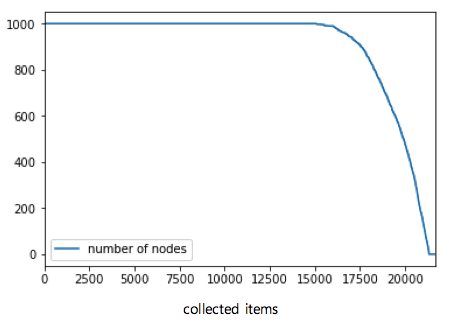
\includegraphics[width=0.7\columnwidth]{figs/figure_06_nr.png}
    \caption{Number of IPs reduced by detection}
    \label{fig:fig7}
\end{figure}

Detection performance of LTM against distributed crawlers can be vary depending on the number of items and long-tail ratio. Since this simulation is based on old NASA traffic data(1995), total number of items were quite small compared to modern web services. If there is a service with 10 times data and equal distribution, that service could detect a distributed crawler consists of 2000 nodes.
\end{itemize}


\begin{table}[H]
  \caption{Experiment Data}
    \begin{tabular}{| l | l | l | l | l | }
    \hline
    & Threshold & Max Node & False Positive \\ \hline
    LTM & 10 & 426 & 0.1239\% \\ 
    LTM & 20 & 222 & 0.0275\% \\ 
    LTM & 35 & 128 & 0.0046\% \\ 
    FBA & 10 & 573 & 8.8064\% \\
    FBA & 20 & 299 & 2.8819\% \\ 
    FBA & 35 & 173 & 0.8903\% \\ 
    FBA & 100 & 60 & 0.0367\% \\ \hline
    \end{tabular}
\end{table}

In the experiments, we compared the detection capability and the false positives between LTM and FBA with equal threshold and environments.

\begin{figure}[H]
    \centering
    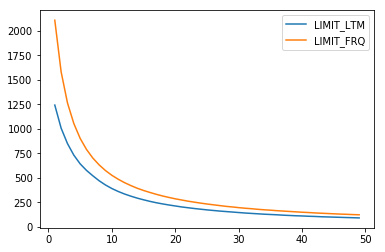
\includegraphics[width=0.85\columnwidth]{figs/figure_limit_compare.png}
    \caption{Number of Detectable Crawler Nodes}
    \label{fig:my_label}
\end{figure}

Since LTM uses long-tail region instead of entire items, FBA detects more crawler nodes with equivalent threshold as figure 8. But as shown in the following figure, it is meaningless to simply compare the detection results without considering false positives.

\begin{figure}[H]
    \centering
    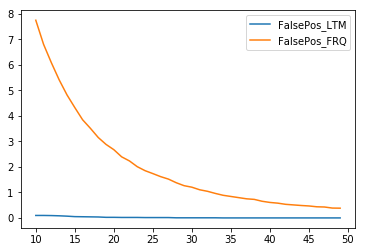
\includegraphics[width=0.85\columnwidth]{figs/figure_fp_compare_01.png}
    \caption{False Positive: 1 to 50}
    \label{fig:my_label}
\end{figure}

As we can verify from figure 8 and 9, as threshold in x-axis increases false positive and number of detectable crawler nodes are both decrease. In the case of LTM, we can verify that the false positive value is less than 0.15 \% from the low threshold region of less than 10.

\begin{figure}[H]
    \centering
    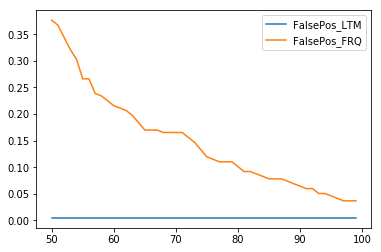
\includegraphics[width=0.85\columnwidth]{figs/figure_fp_compare_02.png}
    \caption{False Positive: 50 to 100}
    \label{fig:my_label}
\end{figure}

 However, in case of FBA, the threshold should be set to 76 or more to have similar false positive error performance by trading off the detection performance.\\

\begin{figure}[H]
    \centering
    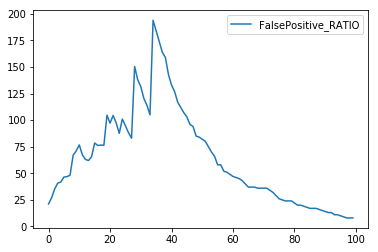
\includegraphics[width=0.85\columnwidth]{figs/figure_fp_ratio.png}
    \caption{Number of Detectable Crawler Nodes}
    \label{fig:my_label}
\end{figure}

In this experiment, LTM reached the minimum false positive error rate of 0.0046\% when FBA reached only 0.0367\% which is 798\% larger than the best score of LTM. This means within the similar level of false positive, LTM performs 400\~500\% better detection score than classic FBA method. And even though FBA trade off the detection score, FBA generates 798\% times more false positive error. When we set the threshold to 35 which is the value that LTM reached the minimum false positive, FBA generated 19400\% times more false positive than LTM.


%
% CONCLUSION
%
\section{CONCLUSION}
In this paper, we introduced LTM(Long-tail Threshold Model) a node reducing method that identifies the IP set of distributed crawlers and gradually reduces IP by using the long-tail region.
By simulating with the real web traffic data, LTM effectively identified distributed crawler and showed a very low level of false positive error.
Web crawling against the term of web service or impairs quality is a serious security threat. And considering that there are some crawler developer using distributed crawler proxy service for illegal purposes, LTM could improve web service data security.


%
% FUTURE WORKS
%
\section{FUTURE WORKS}
Web traffic generally tends to generate traffic bursts at certain times. [1] Although the experiment of this paper is based on actual traffic log, since the time point of the data used in the experiment is one month, it does not include cases where a new item is added or an issue occurs and a traffic burst occurs.
In order to apply the results of this paper more securely to actual services, it is necessary to study whether the item movement level and threshold value of long-tail area can be maintained based on actual traffic data for traffic burst occurrence cases.



% Bibliography
\nocite{*}
\bibliographystyle{ACM-Reference-Format}
\bibliography{exbib}


\end{document}
